% !TEX program = xelatex

\documentclass[compress, aspectratio=169]{beamer}
\usepackage[english]{babel}

\usepackage{graphicx}
\usepackage{amsmath}
\usepackage[export]{adjustbox}
\usepackage[absolute,overlay]{textpos}
\usepackage{hyperref}
\usepackage{pgfplots}

\usepackage{tikz}
\tikzset{
  invisible/.style={opacity=0},
  visible on/.style={alt={#1{}{invisible}}},
  alt/.code args={<#1>#2#3}{%
    \alt<#1>{\pgfkeysalso{#2}}{\pgfkeysalso{#3}} % \pgfkeysalso doesn't change the path
  },
}
\usetikzlibrary{pgfplots.groupplots, shapes.geometric, arrows}

\tikzstyle{startstop} = [rectangle, rounded corners, minimum width=3cm, minimum height=1cm,text centered, draw=black, fill=green!30]
\tikzstyle{process} = [rectangle, minimum width=3cm, minimum height=1cm, text centered, draw=black, fill=orange!30]
\tikzstyle{arrow} = [thick,->,>=stealth]


\newcommand\mybox[2][]{\tikz[overlay]\node[fill=green!20,inner sep=2pt, anchor=text, rectangle, rounded corners=1mm,#1] {#2};\phantom{#2}}
\newcommand\myboxblue[2][]{\tikz[overlay]\node[fill=blue!12,inner sep=2pt, anchor=text, rectangle, rounded corners=1mm,#1] {#2};\phantom{#2}}

\usetikzlibrary{shapes.misc}
% \usetikzlibrary{external}
% \tikzexternalize[optimize = false]
\usepackage{pgfplots}
\usetikzlibrary{calc}

\pgfplotsset{compat=1.14}
\usepackage{booktabs}
\usepackage{siunitx}
\DeclareSIUnit[]\dyne{dyn}

% \tikzexternalize[prefix=tikz/,up to date check=diff]

\usetheme[nobackground,logo]{boz}
\newcommand{\putat}[3]{\begin{picture}(0,0)(0,0)\put(#1,#2){#3}\end{picture}}

\usetikzlibrary{backgrounds}
\title{\Large \Medium Post-processing Cactus simulations with Python}
\subtitle{\tiny .}
\date{June 16, 2022 \vspace*{-0.25cm}}
\author{{Gabriele Bozzola}}
\institute{Department of Astronomy and Steward Observatory, \\
  University of Arizona}
\conference{}

\begin{document}

{
  \usebackgroundtemplate{\begin{picture}(100,0)\put(250,-190){
\includegraphics[width=6cm]{logo_post}}\end{picture}}
  \begin{frame}
    \titlepage
  \end{frame}
}

\begin{frame}
  \frametitle{Plan for the day}
  \centering
    \begin{enumerate}
      \item A brief general introduction on \texttt{kuibit}
      \item Installing and setting up \texttt{kuibit}
      \item Exploring examples
      \item Questions and break
      \item Developing a script for a new analysis
    \end{enumerate}
    All the material is public, focus on understanding and ask questions

    \url{https://github.com/Sbozzolo/kuibit_ETUIdaho}
\end{frame}

\begin{frame}
  \frametitle{Kuibit is a Python library for post-processing simulations}
  \centering

  Post-processing = visualization \& quantitative analysis \\[1cm]

     \begin{columns}
       \begin{column}{0.5\linewidth}
         \centering
         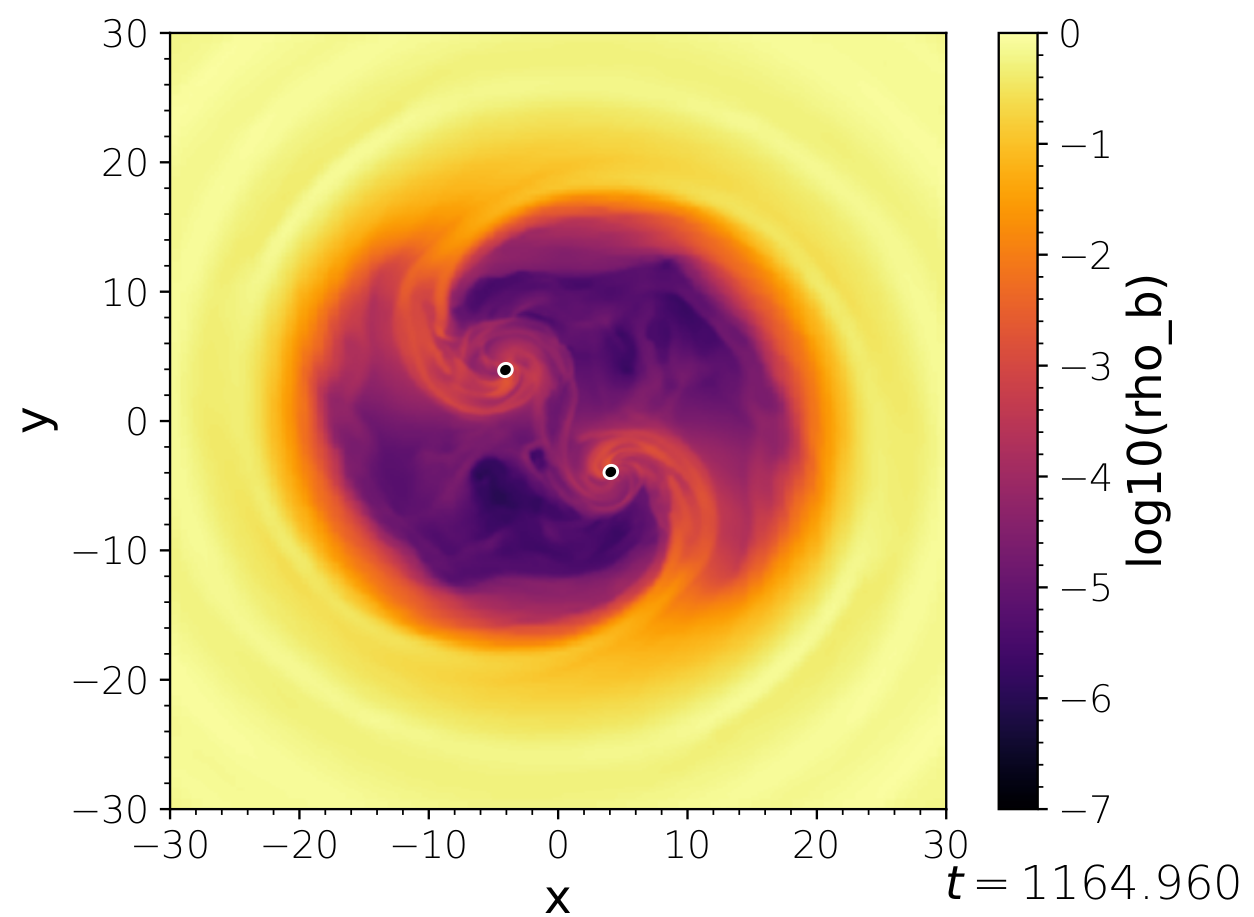
\includegraphics[width=0.8\columnwidth]{grid2D}
       \end{column}
       \begin{column}{0.5\linewidth}
         \hspace{-1cm}
         % This file was created by matplotlib2tikz v0.7.5.
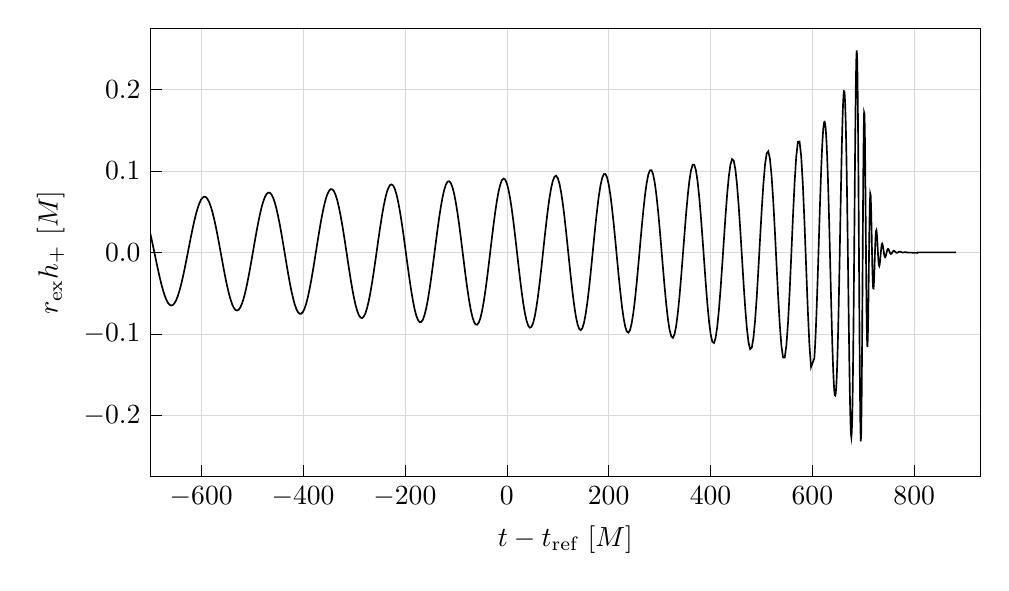
\begin{tikzpicture}

\begin{axis}[
legend cell align={left},
legend style={at={(0.01,0.99)}, anchor=north west, line width=0.25pt},
tick pos=left,
% xlabel={\(\displaystyle t - t_{\SI{30}{\Hz}}~[\si{\admmass}]\)},
xlabel={\(\displaystyle t - t_{\text{ref}}~[M]\)},
xmin=-700, xmax=930,
xtick style={color=black},
grid=both,
y tick label style={
  /pgf/number format/.cd,
  fixed,
  fixed zerofill,
  precision=1,
  /tikz/.cd
},
width = \linewidth,
height = 0.6\linewidth,
% legend columns=2,
grid style={line width=.2pt, draw=gray!30},
minor grid style={line width=.05pt, draw=gray!15},
ylabel={\(\displaystyle r_{\text{ex}} h_+~[M]\)},
ymin=-0.275, ymax=0.275,
ytick style={color=black},
    grid=both,
    grid style={line width=.2pt, draw=gray!30},
    minor grid style={line width=.05pt, draw=gray!8},
    legend cell align={left},
    ytick style={color=black},
]
\addplot [semithick, black]
table {%
-1233.5 0.000680684
-1230.27 0.000344251
-1227.04 -3.01605e-05
-1223.81 -0.000438232
-1220.59 -0.000873609
-1217.36 -0.00132789
-1214.13 -0.00179064
-1210.9 -0.00224943
-1207.67 -0.00269002
-1204.44 -0.00309638
-1201.21 -0.0034511
-1197.98 -0.00373531
-1194.75 -0.00392944
-1191.52 -0.00401327
-1188.29 -0.00396636
-1185.07 -0.00376847
-1181.84 -0.00340031
-1178.61 -0.00284349
-1175.38 -0.00208158
-1172.15 -0.0011004
-1168.92 0.000111625
-1165.69 0.00156238
-1162.46 0.00325588
-1159.23 0.00519152
-1156 0.00736824
-1152.77 0.00973166
-1149.55 0.0123356
-1146.32 0.0151242
-1143.09 0.0179522
-1139.86 0.0208597
-1136.63 0.0236324
-1133.4 0.026104
-1130.17 0.0278684
-1126.94 0.0282026
-1123.71 0.0258373
-1120.48 0.0194824
-1117.26 0.0114661
-1114.03 0.00745926
-1110.8 0.0078412
-1107.57 0.00840449
-1104.34 0.00557603
-1101.11 -3.66783e-05
-1097.88 -0.00637596
-1094.65 -0.0133012
-1091.42 -0.0204632
-1088.19 -0.0270072
-1084.96 -0.0324984
-1081.74 -0.0369781
-1078.51 -0.0406286
-1075.28 -0.0432745
-1072.05 -0.0448422
-1068.82 -0.0453782
-1065.59 -0.0448518
-1062.36 -0.0432675
-1059.13 -0.0407017
-1055.9 -0.0371933
-1052.67 -0.0328186
-1049.45 -0.0276653
-1046.22 -0.0218705
-1042.99 -0.0155392
-1039.76 -0.00877306
-1036.53 -0.00177555
-1033.3 0.0053509
-1030.07 0.0124228
-1026.84 0.0193061
-1023.61 0.0258424
-1020.38 0.0319128
-1017.15 0.0373836
-1013.93 0.0421097
-1010.7 0.0460211
-1007.47 0.0489809
-1004.24 0.0509738
-1001.01 0.0518993
-997.78 0.0517968
-994.551 0.0505722
-991.322 0.0483252
-988.093 0.045002
-984.864 0.0407743
-981.635 0.0356141
-978.406 0.0297251
-975.177 0.0231251
-971.948 0.0160369
-968.718 0.00853052
-965.489 0.000811364
-962.26 -0.00697236
-959.031 -0.0146691
-955.802 -0.0220972
-952.573 -0.0291013
-949.344 -0.0355479
-946.115 -0.0412841
-942.886 -0.0461821
-939.657 -0.0501336
-936.428 -0.0530539
-933.199 -0.0548476
-929.97 -0.0554745
-926.741 -0.0549303
-923.512 -0.0532073
-920.283 -0.0503519
-917.053 -0.0463947
-913.824 -0.0414369
-910.595 -0.0355448
-907.366 -0.0288785
-904.137 -0.0215421
-900.908 -0.0137213
-897.679 -0.00555668
-894.45 0.00276793
-891.221 0.0110664
-887.992 0.0191807
-884.763 0.0268901
-881.534 0.0340852
-878.305 0.0405452
-875.076 0.0461458
-871.847 0.0507835
-868.618 0.0543135
-865.388 0.056689
-862.159 0.0578462
-858.93 0.0576953
-855.701 0.0563211
-852.472 0.0535873
-849.243 0.0499706
-846.014 0.0449358
-842.785 0.039113
-839.556 0.0323036
-836.327 0.0247374
-833.098 0.0165951
-829.869 0.00809005
-826.64 -0.000611751
-823.411 -0.00929434
-820.182 -0.0179229
-816.953 -0.0261867
-813.724 -0.0337313
-810.494 -0.0407507
-807.265 -0.0467359
-804.036 -0.0518674
-800.807 -0.0557419
-797.578 -0.0584019
-794.349 -0.0598315
-791.12 -0.0598855
-787.891 -0.0586367
-784.662 -0.0560366
-781.433 -0.0522474
-778.204 -0.0471757
-774.975 -0.0411238
-771.746 -0.0340668
-768.517 -0.026265
-765.288 -0.017795
-762.059 -0.00893025
-758.829 0.000223384
-755.6 0.00935483
-752.371 0.0183328
-749.142 0.0269824
-745.913 0.0349636
-742.684 0.0422816
-739.455 0.048597
-736.226 0.0538781
-732.997 0.0579398
-729.768 0.0607028
-726.539 0.0620472
-723.31 0.0620663
-720.081 0.0605947
-716.852 0.0577539
-713.623 0.0535357
-710.394 0.0481158
-707.164 0.041505
-703.935 0.0339305
-700.706 0.0255419
-697.477 0.0164908
-694.248 0.00703216
-691.019 -0.00266284
-687.79 -0.0123229
-684.561 -0.0217572
-681.332 -0.0307747
-678.103 -0.0390284
-674.874 -0.0465379
-671.645 -0.0528534
-668.416 -0.0580912
-665.187 -0.0619084
-661.958 -0.0642938
-658.729 -0.0651788
-655.499 -0.0644786
-652.27 -0.0622871
-649.041 -0.0585476
-645.812 -0.0534816
-642.583 -0.0470223
-639.354 -0.0393931
-636.125 -0.0307785
-632.896 -0.0213244
-629.667 -0.0113426
-626.438 -0.00107048
-623.209 0.00924343
-619.98 0.0195034
-616.751 0.0292662
-613.522 0.0384669
-610.293 0.0467078
-607.064 0.0539603
-603.835 0.0597385
-600.605 0.0642238
-597.376 0.0671204
-594.147 0.0682974
-590.918 0.0678458
-587.689 0.0655737
-584.46 0.0618396
-581.231 0.0564484
-578.002 0.0497109
-574.773 0.0415769
-571.544 0.0323584
-568.315 0.0222798
-565.086 0.0115973
-561.857 0.000496473
-558.628 -0.0105317
-555.399 -0.0214027
-552.17 -0.0318689
-548.94 -0.0415604
-545.711 -0.050089
-542.482 -0.0575108
-539.253 -0.0635451
-536.024 -0.0678906
-532.795 -0.0704875
-529.566 -0.0713214
-526.337 -0.0703664
-523.108 -0.0674509
-519.879 -0.0628638
-516.65 -0.0565986
-513.421 -0.0488682
-510.192 -0.0398444
-506.963 -0.0297321
-503.734 -0.0187733
-500.505 -0.00730649
-497.275 0.00438346
-494.046 0.0160439
-490.817 0.0272726
-487.588 0.0378756
-484.359 0.0474577
-481.13 0.0559239
-477.901 0.062846
-474.672 0.0681574
-471.443 0.0717156
-468.214 0.0733519
-464.985 0.0730907
-461.756 0.0707991
-458.527 0.066764
-455.298 0.0607557
-452.069 0.0532359
-448.84 0.0441816
-445.61 0.0340152
-442.381 0.0228056
-439.152 0.0109995
-435.923 -0.00119441
-432.694 -0.0133604
-429.465 -0.0252447
-426.236 -0.036516
-423.007 -0.0467607
-419.778 -0.0557298
-416.549 -0.0633483
-413.32 -0.069195
-410.091 -0.073186
-406.862 -0.0752423
-403.633 -0.0752549
-400.404 -0.0731418
-397.175 -0.0690935
-393.946 -0.0630871
-390.716 -0.0553364
-387.487 -0.0460618
-384.258 -0.0354957
-381.029 -0.0238768
-377.8 -0.0115221
-374.571 0.00114999
-371.342 0.0139008
-368.113 0.0262408
-364.884 0.0379596
-361.655 0.0486302
-358.426 0.0580556
-355.197 0.065809
-351.968 0.0717793
-348.739 0.0757514
-345.51 0.0776229
-342.281 0.077247
-339.051 0.0747522
-335.822 0.0700611
-332.593 0.0634259
-329.364 0.054838
-326.135 0.0447601
-322.906 0.0332838
-319.677 0.0207617
-316.448 0.00764004
-313.219 -0.00584273
-309.99 -0.019152
-306.761 -0.0320624
-303.532 -0.0440599
-300.303 -0.054796
-297.074 -0.0640459
-293.845 -0.0713851
-290.616 -0.0767758
-287.386 -0.079806
-284.157 -0.0806015
-280.928 -0.0789021
-277.699 -0.0749301
-274.47 -0.068667
-271.241 -0.0603
-268.012 -0.0501826
-264.783 -0.038381
-261.554 -0.0254426
-258.325 -0.0116055
-255.096 0.00262153
-251.867 0.0168606
-248.638 0.0306404
-245.409 0.0435826
-242.18 0.0552352
-238.951 0.0652362
-235.721 0.0733071
-232.492 0.0791248
-229.263 0.082543
-226.034 0.0834021
-222.805 0.0816965
-219.576 0.0774192
-216.347 0.0706338
-213.118 0.061692
-209.889 0.0507007
-206.66 0.0381302
-203.431 0.0242689
-200.202 0.00958967
-196.973 -0.00547412
-193.744 -0.0204785
-190.515 -0.0348185
-187.286 -0.0482075
-184.057 -0.0599938
-180.827 -0.0700037
-177.598 -0.0777182
-174.369 -0.0829373
-171.14 -0.0856042
-167.911 -0.08535
-164.682 -0.082543
-161.453 -0.0768016
-158.224 -0.0687175
-154.995 -0.0582039
-151.766 -0.04586
-148.537 -0.0319255
-145.308 -0.0169153
-142.079 -0.00127315
-138.85 0.0144495
-135.621 0.0297474
-132.392 0.0441593
-129.162 0.0570194
-125.933 0.0681643
-122.704 0.0769795
-119.475 0.0832173
-116.246 0.0867182
-113.017 0.0873294
-109.788 0.0849614
-106.559 0.079736
-103.33 0.0717793
-100.101 0.0613877
-96.8718 0.04883
-93.6428 0.0345594
-90.4137 0.019103
-87.1847 0.0028911
-83.9556 -0.0134272
-80.7265 -0.0293706
-77.4975 -0.0443254
-74.2684 -0.0577997
-71.0394 -0.0693477
-67.8103 -0.0784309
-64.5812 -0.0848788
-61.3522 -0.0884049
-58.1231 -0.0887171
-54.894 -0.0860628
-51.665 -0.0802514
-48.4359 -0.0716204
-45.2069 -0.0603744
-41.9778 -0.0469822
-38.7487 -0.0318294
-35.5197 -0.0154952
-32.2906 0.00147193
-29.0616 0.0184136
-25.8325 0.0347536
-22.6034 0.0499687
-19.3744 0.0633672
-16.1453 0.0744848
-12.9162 0.0829373
-9.68718 0.0884244
-6.45812 0.0906013
-3.22906 0.0893725
0 0.084904
3.22906 0.0772728
6.45812 0.066687
9.68718 0.0535344
12.9162 0.0382696
16.1453 0.021551
19.3744 0.0039521
22.6034 -0.0140147
25.8325 -0.0313603
29.0616 -0.0476193
32.2906 -0.0621859
35.5197 -0.0743447
38.7487 -0.0836374
41.9778 -0.0897926
45.2069 -0.0923643
48.4359 -0.0913715
51.665 -0.0867693
54.894 -0.0786536
58.1231 -0.0674004
61.3522 -0.0534492
64.5812 -0.0372137
67.8103 -0.0194397
71.0394 -0.000784057
74.2684 0.0179458
77.4975 0.0360195
80.7265 0.0526701
83.9556 0.0673683
87.1847 0.0791563
90.4137 0.0878195
93.6428 0.0928159
96.8718 0.0939936
100.101 0.0911614
103.33 0.0845224
106.559 0.0742684
109.788 0.0608295
113.017 0.0447156
116.246 0.0266119
119.475 0.00734597
122.704 -0.0122974
125.933 -0.0315977
129.162 -0.0494913
132.392 -0.0652678
135.621 -0.0784057
138.85 -0.087928
142.079 -0.0937136
145.308 -0.0953492
148.537 -0.0927585
151.766 -0.0859354
154.995 -0.0752739
158.224 -0.0612235
161.453 -0.0442897
164.682 -0.0253147
167.911 -0.00508407
171.14 0.0154628
174.369 0.0353028
177.598 0.0536726
180.827 0.0696088
184.057 0.0823008
187.286 0.0913014
190.515 0.095973
193.744 0.0961194
196.973 0.0917852
200.202 0.083071
203.431 0.0702774
206.66 0.0541124
209.889 0.0352857
213.118 0.0145946
216.347 -0.00681385
219.576 -0.0281128
222.805 -0.0480439
226.034 -0.0657263
229.263 -0.080334
232.492 -0.0909766
235.721 -0.0971128
238.951 -0.0984558
242.18 -0.0948723
245.409 -0.0863876
248.638 -0.0735998
251.867 -0.0567915
255.096 -0.0371213
258.325 -0.0153673
261.554 0.00733708
264.783 0.0298728
268.012 0.0509165
271.241 0.0694246
274.47 0.0843887
277.699 0.0950313
280.928 0.100607
284.157 0.100798
287.386 0.0955725
290.616 0.0850889
293.845 0.0698636
297.074 0.0506918
300.303 0.0285214
303.532 0.00462807
306.761 -0.019751
309.99 -0.0432166
313.219 -0.0643575
316.448 -0.0821545
319.677 -0.0952161
322.906 -0.102905
326.135 -0.104853
329.364 -0.100454
332.593 -0.0901875
335.822 -0.0745289
339.051 -0.0542722
342.281 -0.0305678
345.51 -0.00474246
348.739 0.0214384
351.968 0.0466289
355.197 0.0691698
358.426 0.0875079
361.655 0.1006
364.884 0.107443
368.113 0.107488
371.342 0.100728
374.571 0.0873609
377.8 0.0682085
381.029 0.0444336
384.258 0.0175569
387.487 -0.0107036
390.716 -0.0384937
393.946 -0.0639885
397.175 -0.0853304
400.404 -0.100938
403.633 -0.109779
406.862 -0.111148
410.091 -0.104617
413.32 -0.0907028
416.549 -0.0702579
419.778 -0.0445195
423.007 -0.015375
426.236 0.0151604
429.465 0.0449256
432.694 0.0715056
435.923 0.0931408
439.152 0.107832
442.381 0.114509
445.61 0.112478
448.84 0.10167
452.069 0.0828357
455.298 0.0572052
458.527 0.0267806
461.756 -0.0061382
464.985 -0.0389488
468.214 -0.0689276
471.443 -0.0935798
474.672 -0.110639
477.901 -0.118684
481.13 -0.116653
484.359 -0.104496
487.588 -0.0831158
490.817 -0.0541691
494.046 -0.019926
497.275 0.0165741
500.505 0.0520692
503.734 0.0832621
506.963 0.107202
510.192 0.121332
513.421 0.124043
516.65 0.114801
519.879 0.094121
523.108 0.0637337
526.337 0.0264095
529.566 -0.0142706
532.795 -0.0541525
536.024 -0.0890546
539.253 -0.11503
542.482 -0.128938
545.711 -0.128906
548.94 -0.114229
552.17 -0.0863365
555.399 -0.0477454
558.628 -0.00272841
561.857 0.0435889
565.086 0.0855474
568.315 0.117653
571.544 0.135507
574.773 0.135991
578.002 0.118296
581.231 0.0840323
584.46 0.0370272
587.689 -0.0164532
590.918 -0.0691824
594.147 -0.113006
597.376 -0.140618
603.835 -0.129912
604.642 -0.121943
605.449 -0.112637
606.256 -0.102058
607.064 -0.0903086
607.871 -0.0774759
608.678 -0.0636895
609.485 -0.0490757
610.293 -0.0337873
611.1 -0.0179827
611.907 -0.00182978
612.714 0.0144972
613.522 0.0308167
614.329 0.0469415
615.136 0.0626786
615.943 0.077833
616.751 0.0922243
617.558 0.105654
618.365 0.117958
619.173 0.12897
619.98 0.138537
620.787 0.146519
621.594 0.152788
622.402 0.157218
623.209 0.15972
624.016 0.160204
624.823 0.158619
625.631 0.154934
626.438 0.149166
627.245 0.141344
628.052 0.131542
628.86 0.119842
629.667 0.106374
630.474 0.0912819
631.282 0.0747453
632.089 0.056957
632.896 0.0381398
633.703 0.0185276
634.511 -0.00161858
635.318 -0.0220157
636.125 -0.042358
636.932 -0.0623304
637.74 -0.0816132
638.547 -0.099894
639.354 -0.11687
640.161 -0.132242
640.969 -0.14571
641.776 -0.157008
642.583 -0.165875
643.391 -0.172081
644.198 -0.175435
645.005 -0.175811
645.812 -0.173106
646.62 -0.167275
647.427 -0.158332
648.234 -0.146334
649.041 -0.131421
649.849 -0.113764
650.656 -0.093612
651.463 -0.0712703
652.27 -0.0470898
653.078 -0.0214931
653.885 0.00505384
654.692 0.0320344
655.499 0.05889
656.307 0.0850315
657.114 0.109843
657.921 0.132719
658.729 0.153049
659.536 0.170235
660.343 0.183736
661.15 0.193054
661.958 0.197783
662.765 0.19758
663.572 0.192214
664.379 0.181584
665.187 0.165697
665.994 0.144736
666.801 0.119021
667.608 0.0890672
668.416 0.0555528
669.223 0.0193372
670.03 -0.0185639
670.838 -0.0569907
671.645 -0.0946623
672.452 -0.130205
673.259 -0.162183
674.067 -0.189152
674.874 -0.209718
675.681 -0.222601
676.488 -0.226713
677.296 -0.221245
678.103 -0.205727
678.91 -0.18012
679.717 -0.144915
680.525 -0.101148
681.332 -0.0505008
682.139 0.00475023
682.947 0.0617397
683.754 0.117112
684.561 0.167154
685.368 0.208006
686.176 0.235942
686.983 0.247743
687.79 0.241079
688.597 0.215014
689.405 0.170337
690.212 0.109824
691.019 0.0382722
691.826 -0.0377795
692.634 -0.110581
693.441 -0.171947
694.248 -0.214288
695.055 -0.231728
695.863 -0.221271
696.67 -0.183678
697.477 -0.123821
698.285 -0.0501399
699.092 0.0266304
699.899 0.0952665
700.706 0.145939
701.514 0.171769
702.321 0.169904
703.128 0.14205
703.935 0.0941911
704.743 0.035525
705.55 -0.023381
706.357 -0.0726517
707.164 -0.104897
707.972 -0.116272
708.779 -0.106826
709.586 -0.0801751
710.394 -0.0426737
711.201 -0.00205319
712.008 0.0341469
712.815 0.0600027
713.623 0.0721231
714.43 0.0699652
715.237 0.0555662
716.044 0.0329567
716.852 0.0072002
717.659 -0.0166512
718.466 -0.034518
719.273 -0.0439282
720.081 -0.0442516
720.888 -0.0365644
721.695 -0.023255
722.503 -0.00743763
723.31 0.00770117
724.117 0.0195027
724.924 0.0262574
725.732 0.0273859
726.539 0.0233969
727.346 0.0156664
728.153 0.00608187
728.961 -0.0033695
729.768 -0.0109805
730.575 -0.0156003
731.382 -0.0167682
732.19 -0.0147072
732.997 -0.0102001
733.804 -0.0043764
734.612 0.00154023
735.419 0.00646572
736.226 0.00963427
737.033 0.010694
737.841 0.00971892
738.648 0.00714482
739.455 0.00364594
740.262 -1.86135e-05
741.07 -0.0031548
741.877 -0.00525186
742.684 -0.00605335
743.491 -0.0055747
744.299 -0.00406699
745.106 -0.00193913
745.913 0.000339923
746.72 0.002336
747.528 0.00372347
748.335 0.00432961
749.142 0.00414675
749.95 0.00331177
750.757 0.00206281
751.564 0.000682148
752.371 -0.000560359
753.179 -0.00145475
753.986 -0.00188153
754.793 -0.00182163
755.6 -0.0013475
756.408 -0.000598054
757.215 0.00025442
758.022 0.00104025
758.829 0.00162368
759.637 0.00192386
760.444 0.00192214
761.251 0.00165678
762.059 0.00120816
762.866 0.000679095
763.673 0.000174169
764.48 -0.000219272
765.288 -0.000444903
766.095 -0.000484239
766.902 -0.000355186
767.709 -0.000104082
768.517 0.000205854
769.324 0.000507592
770.131 0.000743447
770.938 0.00087571
771.746 0.000891435
772.553 0.000800924
773.36 0.000631527
774.168 0.000420003
774.975 0.000204995
775.782 2.12831e-05
776.589 -0.000104916
777.397 -0.000159695
778.204 -0.000143954
779.011 -7.31986e-05
779.818 2.65648e-05
780.626 0.000126233
781.433 0.000201392
782.24 0.000237292
783.047 0.000229475
783.855 0.000181412
784.662 0.000101568
785.469 1.92481e-06
786.276 -0.000102828
787.084 -0.000197299
787.891 -0.000268984
788.698 -0.000311509
789.506 -0.000325372
790.313 -0.000316302
791.12 -0.000293025
791.927 -0.000266018
792.735 -0.000246489
793.542 -0.000244076
794.349 -0.00026377
795.156 -0.000304329
795.964 -0.000359419
796.771 -0.00042053
797.578 -0.000479669
798.385 -0.0005308
799.193 -0.000570378
800 -0.000597442
800.807 -0.000613221
801.615 -0.000620179
802.422 -0.000621273
803.229 -0.000619994
804.036 -0.000620478
804.844 -0.000626703
805.651 -0.000641159
806.458 -0.00066407
807.265 0
881.534 0
};
\end{axis}
\end{tikzpicture}

       \end{column}
     \end{columns}
     \hfill\\[1cm]

    {\Medium kuibit takes care of the low-level details and lets you focus
       on science}
\end{frame}

\begin{frame}
  \frametitle{Kuibit has excellent documentation (sbozzolo.github.io/kuibit)}
  \centering
  \begin{columns}
    \begin{column}{0.5\linewidth}
      \centering
      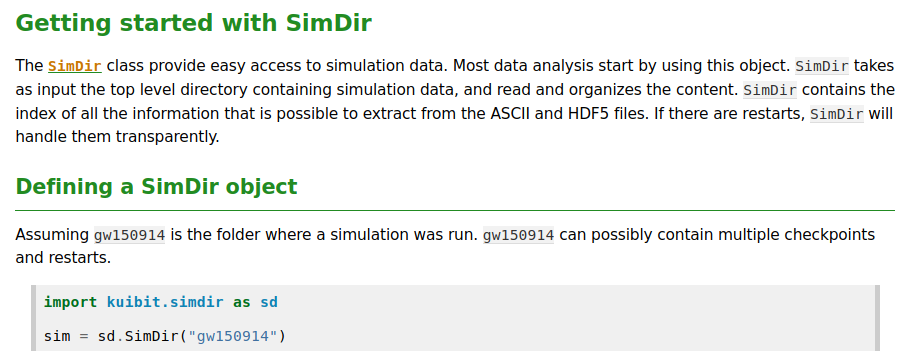
\includegraphics[width=\columnwidth]{usage}
      {\Medium USAGE}\\[0.2cm]
      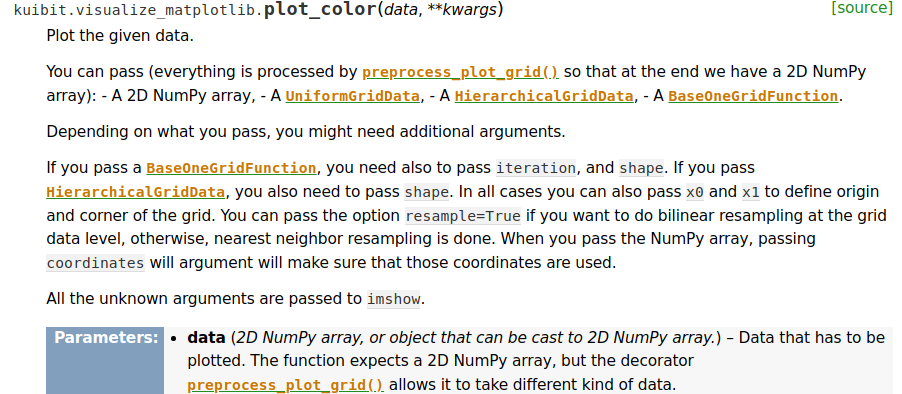
\includegraphics[width=\columnwidth]{apis}
      {\Medium APIs}
    \end{column}
    \begin{column}{0.5\linewidth}
      \centering
      \hfill \\[0.1cm]
      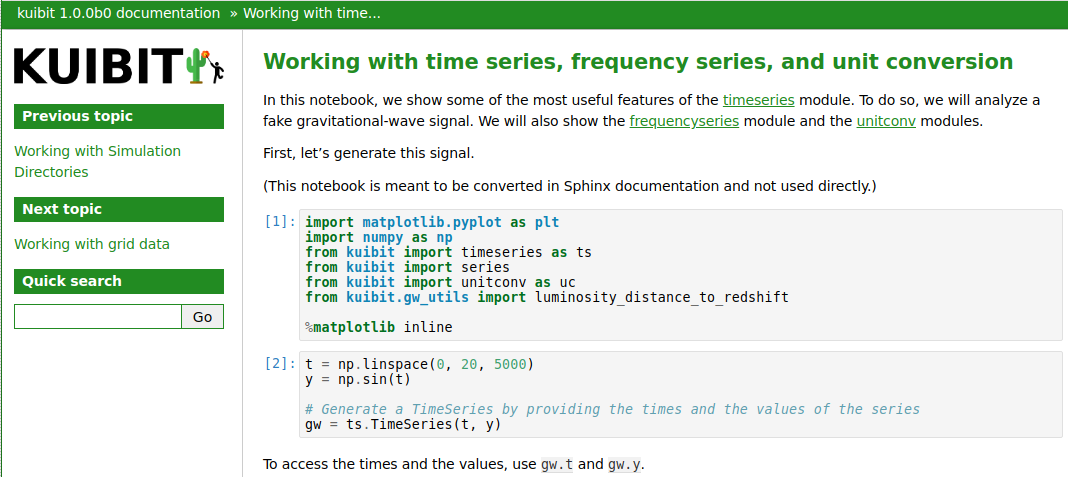
\includegraphics[width=\columnwidth, height=0.4\columnwidth]{tut}
      {\Medium TUTORIALS}
      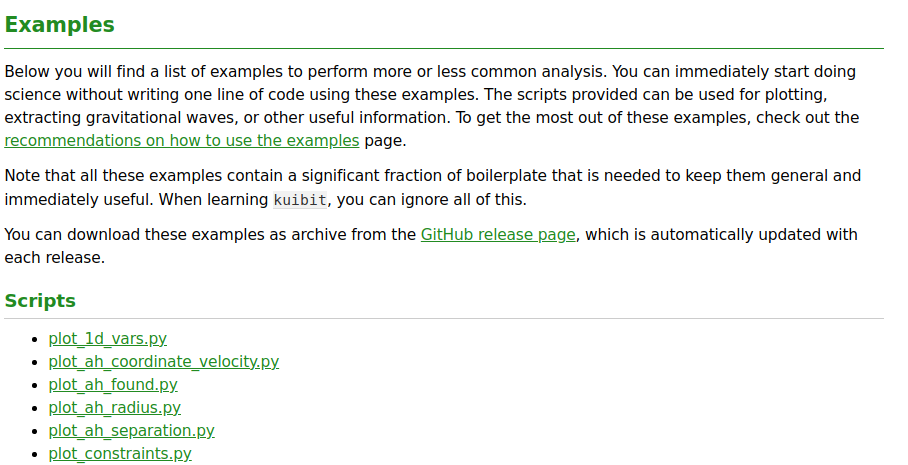
\includegraphics[width=\columnwidth]{examples}
      {\Medium EXAMPLES}
    \end{column}
  \end{columns}
\end{frame}

\begin{frame}
  \frametitle{How to get help?}
  \begin{columns}
    \begin{column}{0.5\linewidth}
      \centering
      
\includegraphics[width=0.4\columnwidth]{email}

      \texttt{gabrielebozzola@email.arizona.edu} \\
      (fast)
    \end{column}
    \begin{column}{0.5\linewidth}
      \centering
      
\includegraphics[width=0.3\columnwidth]{telegram}

      \url{t.me/kuibit} \\
      (fastest) \\[1cm]
    \end{column}
  \end{columns}
      \centering
      
\includegraphics[width=0.2\columnwidth]{profil-circ}

      (instantaneous)
\end{frame}

\begin{frame}
  \frametitle{Structure of the \texttt{kuibit} project}
  \centering
  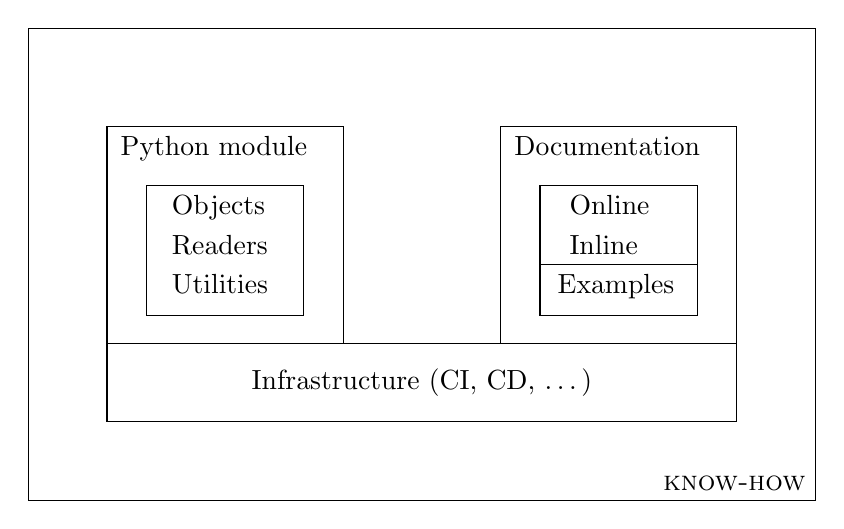
\begin{tikzpicture}
    \draw[visible on=<4->] (0,-1) rectangle (10, 5);

    \node[anchor=south east, visible on=<4->] () at (10, -1) {\textsc{know-how}};

    \draw (1, 1) rectangle (4, 3.75);

    \node[anchor=north west] at (1.05, 3.75) {Python module};

    \draw (1.5, 1.35) rectangle (3.5, 3);
    \node[anchor=north west, align=center] at (1.7, 3) {Objects};
    \node[anchor=north west, align=center] at (1.7, 2.50) {Readers};
    \node[anchor=north west, align=center] at (1.7, 2) {Utilities};

    \draw[visible on=<3->] (1, 1) rectangle (9, 0);
    \node[visible on=<3->] at (5, 0.5) {Infrastructure (CI, CD, \dots)};

    \draw[visible on=<2->] (6, 1) rectangle (9, 3.75);
    \node[anchor=north west, visible on=<2->] at (6.05, 3.75) {Documentation};

    \draw[visible on=<2->] (6.5, 1.35) rectangle (8.5, 3);
    \draw[visible on=<2->] (6.5, 1.35) rectangle (8.5, 2);
    \node[anchor=north west, align=center, visible on=<2->] at (6.75, 3) {Online};
    \node[anchor=north west, align=center, visible on=<2->] at (6.75, 2.50) {Inline};
    \node[anchor=north west, align=center, visible on=<2->] at (6.6, 2) {Examples};
  \end{tikzpicture}

  \texttt{kuibit} is workflow independent
\end{frame}

\begin{frame}
  \frametitle{\texttt{kuibit} has three groups of modules}
  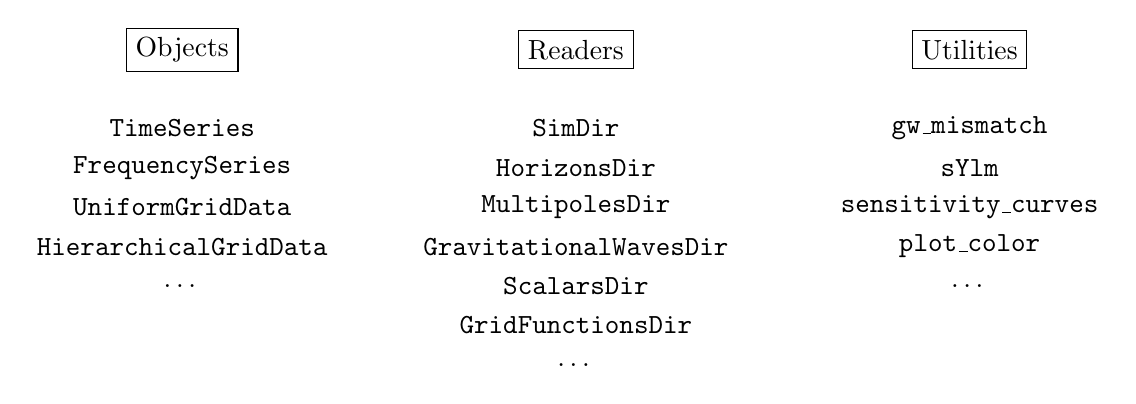
\begin{tikzpicture}
    \node[draw = black, rectangle] (a) at (-3,0) {Objects};

    \node (a) at (-3,-1) {\texttt{TimeSeries}};
    \node (a) at (-3,-1.5) {\texttt{FrequencySeries}};
    \node (a) at (-3,-2) {\texttt{UniformGridData}};
    \node (a) at (-3,-2.5) {\texttt{HierarchicalGridData}};
    \node (a) at (-3,-3) {\dots};
    \pause
    \node[draw = black, rectangle] (b) at (2,0) {Readers};
    \node (a) at (2,-1) {\texttt{SimDir}};
    \node (a) at (2,-1.5) {\texttt{HorizonsDir}};
    \node (a) at (2,-2) {\texttt{MultipolesDir}};
    \node (a) at (2,-2.5) {\texttt{GravitationalWavesDir}};
    \node (a) at (2,-3) {\texttt{ScalarsDir}};
    \node (a) at (2,-3.5) {\texttt{GridFunctionsDir}};
    \node (a) at (2,-4) {\dots};
    \pause
    \node[draw = black, rectangle] (c) at (7,0) {Utilities};
    \node (a) at (7,-1) {\texttt{gw\_mismatch}};
    \node (a) at (7,-1.5) {\texttt{sYlm}};
    \node (a) at (7,-2) {\texttt{sensitivity\_curves}};
    \node (a) at (7,-2.5) {\texttt{plot\_color}};
    \node (a) at (7,-3) {\dots};
  \end{tikzpicture}
\end{frame}

\begin{frame}
  \frametitle{Utilities}

  Convenience functions and useful routines:
  \begin{itemize}
    \item \texttt{gw\_utils} (e.g., \texttt{luminosity\_distance\_to\_redshift},
    \texttt{antenna\_pattern})
    \item \texttt{unitconv} (e.g., from geometrized to physical and viceversa)
    \item \texttt{gw\_mismatch}
    \item \texttt{sensitivity\_curves} (LISA, aLIGO, CE, ET, \dots)
  \end{itemize}

  Helpers for command-line scripts and visualization
  \begin{itemize}
    \item \texttt{argparse\_helper}
    \item \texttt{visualize\_matplotlib}
  \end{itemize}

\end{frame}

\begin{frame}
  \frametitle{Objects (time and frequency series and grid data)}
  \begin{itemize}
    \item High-level abstractions for data and useful methods
    \item E.g., \texttt{TimeSeries} (\texttt{ts(10)}, \texttt{ts1 + np.sin(ts2)})
    \pause
    \item \texttt{UniformGridData} for data on a regular patch
    \item \texttt{HierarchicalGridData} is essentially a collection of
    \texttt{UniformGridData}
    \item \texttt{HierarchicalGridData} cannot be visualized directly and have to be resampled to \texttt{UniformGridData}
  \end{itemize}
\end{frame}

\begin{frame}
  \frametitle{Readers deal with the output mess and present us with an object }
  Readers:
  \begin{itemize}
    \item Find the files associated to what you asked
    \item Deal with reading (e.g., HDF5 files, compressed files, reading correct column)
    \item Clean up the data (e.g., simulation restarts)
  \end{itemize}
  \begin{table}[htbp]
    \centering
    \begin{tabular}[t]{ll}
      \texttt{SimDir} & Main point of entry  (find all the files)\\
  \texttt{*Dir (e.g., GridFunctionsDir)} & Process files from \texttt{SimDir} \\
  \texttt{All* (e.g., AllGridFunctions)} & Organizes in the various variables \\
  \texttt{One* (e.g., OneGridFunction)} & Has one variable (usually indexed by iterations) \\
    \end{tabular}
  \end{table}

  All are dictionary-like that you can print, or get keys, or access with attributes.
\end{frame}

\begin{frame}
  \frametitle{Call for contributions}
  \begin{columns}
    \begin{column}{0.7\linewidth}
      \begin{itemize}
        \item \texttt{kuibit} is a great framework to make your codes available
              to the entire community
        \item Openly developed, accessible, well-commented, easy-to-extend
        \item Great learning opportunity!
        \item \url{github.com/Sbozzolo/kuibit}
      \end{itemize}
    \end{column}
    \begin{column}{0.3\linewidth}
      
\includegraphics[width=\linewidth]{kuibit_learning}
    \end{column}
  \end{columns}
\end{frame}

\begin{frame}
  \centering
  \begin{columns}
    \begin{column}{0.6\linewidth}
      \begin{itemize}
        \item \texttt{kuibit} is published in the Journal of Open-Source Software
        \item Telegram user group/support/announcements at \url{t.me/kuibit}
        \item Feel free to reach me at \texttt{gabrielebozzola@email.arizona.edu}
        \item A \emph{kuibit} is a Tohono O'odham stick to pluck Saguaro's fruit
      \end{itemize}
      \hfill \\[0.5cm]
      \begin{center}
      \emph{Harvest the fruit of your \texttt{Cactus} simulations with \texttt{kuibit}!}
    \end{center}
    \end{column}
    \begin{column}{0.4\linewidth}
      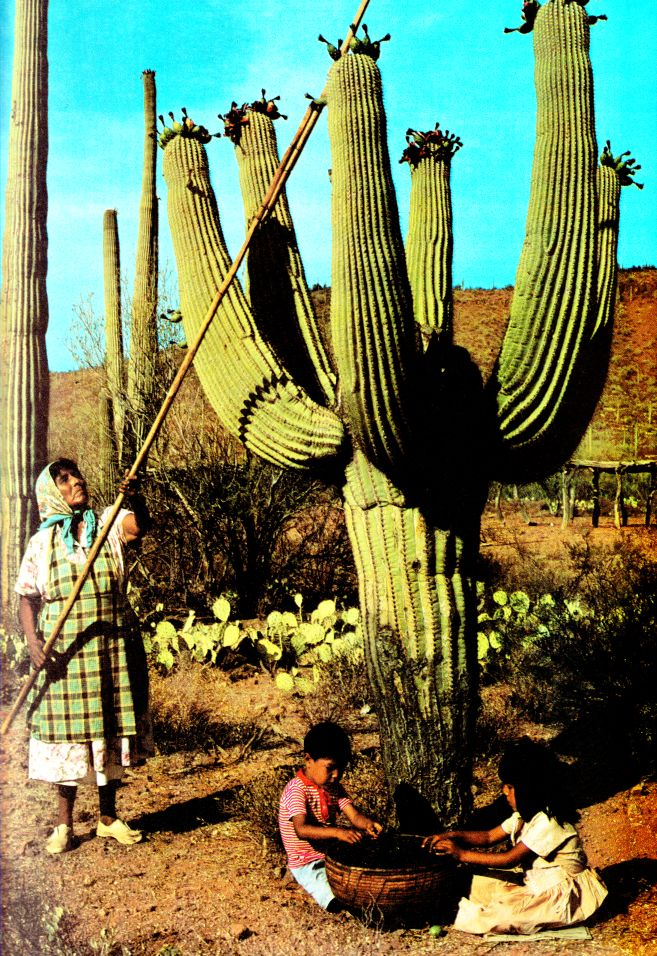
\includegraphics[width=0.85\linewidth]{kuibit}
    \end{column}
  \end{columns}
  \begin{textblock*}{11.5cm}(0.15cm,8.45cm) % {block width} (coords)
    Credits: Wolfgang Kastaun, NumPy, SciPy, h5py, TACC, NSF, NASA
  \end{textblock*}
\end{frame}

\begin{frame}
  \frametitle{Setup}
  \centering
  \url{https://sbozzolo.github.io/kuibit/first_steps.html}
  \url{https://sbozzolo.github.io/kuibit/recommendation_examples.html}
\end{frame}

\end{document}

%%% Local Variables:
%%% mode: latex
%%% TeX-master: t
%%% TeX-engine: xetex
%%% TeX-command-extra-options: "-shell-escape"
%%% End:
